\documentclass[0-protokol.tex]{subfiles}
\begin{document}

\subsection*{Úkol 1}
Následující tabulka obsahuje naměřené hodnoty napětí a proudu při nulové indukci. Pro měření napětí byl použit multimetr \textbf{MY-68}, jako ampérmetr sloužil multimetr \textbf{MY-65} v rozsahu $\SI{20}{mA}$.
\begin{table}[H] 
\centering
\setlength{\tabcolsep}{10pt}
\begin{tabular}{SSSS}                                                                   \toprule
{$U$}       &   {$\sigma_U$}&   {$I_{B=\SI{0}{T}}$} &   {$\sigma_{I_{B=\SI{0}{T}}}$}\\  
{$\si{V}$}  &   {$\si{V}$}  &   {$\si{mA}$}         &   {$\si{mA}$}                 \\  \midrule  
0.236       &   0.003       &   0.496               &   0.007                       \\
0.482       &   0.003       &   1.016               &   0.010                       \\
0.705       &   0.004       &   1.485               &   0.012                       \\
0.964       &   0.005       &   2.038               &   0.015                       \\
1.163       &   0.005       &   2.452               &   0.017                       \\
1.424       &   0.006       &   3.011               &   0.020                       \\
1.637       &   0.007       &   3.469               &   0.022                       \\
1.855       &   0.008       &   3.939               &   0.025                       \\
2.091       &   0.008       &   4.458               &   0.027                       \\
2.323       &   0.009       &   4.967               &   0.030                       \\  \bottomrule    
\end{tabular}


\caption{Naměřené hodnoty napětí a proudu při nulové indukci}
\label{tab:u1}
\end{table}

V následujícím grafu jsou vyobrazeny hodnoty z tabulky \ref{tab:u1}, proložené přímkou se směrnicí $A = \SI{2.129 \pm 0.005 e-3}{}$. 
\begin{figure}[H]
\centering
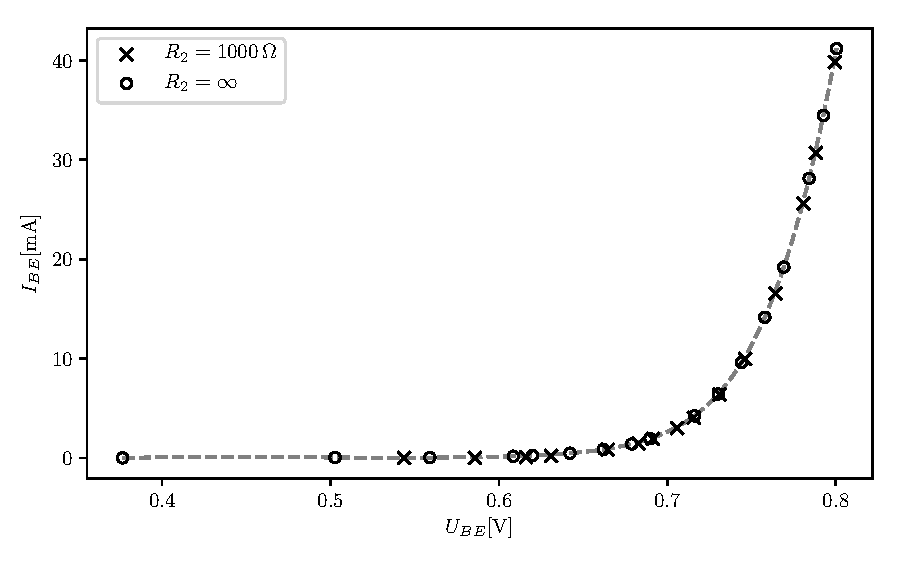
\includegraphics[]{u1}
\caption{Závislost proudu na napětí při nulové indukci}
\label{fig:u1}
\end{figure}

\subsection*{Úkol 2}
V následujících dvou tabulkách lze nalézt naměřené hodnoty proudu napájejícího elektromagnet, napětí na svorkách 5 a 6 při obou polaritách magnetického pole, jakožto i vypočítané hodnoty magnetické indukce podle \eqref{eq:indukce} a Hallova napětí podle \eqref{eq:U_H}. Napětí bylo měřeno multimetrem \textbf{MY-65} při odpovídajících rozsazích, konstantní proud vzorkem byl kontrolován multimetrem \textbf{MY-68} a napájecí proud $I_B$ byl měřen analogovým ampérmetrem třídy přesnosti $\num{0,5}$.
\begin{table}[H] \label{tab:u2_1mA}
\centering
\setlength{\tabcolsep}{4pt}
\begin{tabular}{SSSSSSSSSS}                                                                                                                                               \\ \toprule  
{$I_B$}       & {$\sigma_{I_B}$} & {$U^+$}       & {$\sigma_{U^+}$} & {$U^-$}       & {$\sigma_{U^-}$} & {$B$}         & {$\sigma_B$}  & {$U_H$}       & {$\sigma_{U_H}$} \\
{$[\si{A}]$}  & {$[\si{A}]$}     & {$[\si{mV}]$} & {$[\si{mV}]$}    & {$[\si{mV}]$} & {$[\si{mV}]$}    & {$[\si{T}]$}  & {$[\si{T}]$}  & {$[\si{mV}]$} & {$[\si{mV}]$}    \\ \midrule
0.500         & 0.006            & 17.65         & 0.04             & 9.05          & 0.03             & 0.0490        & 0.0006        & 4.300         & 0.026            \\    
1.000         & 0.006            & 22.37         & 0.04             & 4.53          & 0.03             & 0.0980        & 0.0006        & 8.920         & 0.026            \\    
1.500         & 0.030            & 26.73         & 0.04             & -0.57         & 0.03             & 0.1470        & 0.0029        & 13.650        & 0.026            \\    
2.000         & 0.030            & 31.93         & 0.05             & -4.58         & 0.03             & 0.1960        & 0.0029        & 18.255        & 0.028            \\    
2.500         & 0.030            & 36.37         & 0.05             & -8.93         & 0.03             & 0.2450        & 0.0029        & 22.650        & 0.030            \\    
3.000         & 0.030            & 40.75         & 0.05             & -13.12        & 0.04             & 0.2940        & 0.0029        & 26.935        & 0.031            \\    
3.500         & 0.030            & 44.99         & 0.05             & -16.87        & 0.04             & 0.3430        & 0.0029        & 30.930        & 0.033            \\    
4.000         & 0.030            & 48.63         & 0.05             & -21.04        & 0.04             & 0.3920        & 0.0029        & 34.835        & 0.034            \\ \bottomrule

\end{tabular}

\caption{Naměřené a vypočtené hodnoty pro určení Hallova napětí při konstantním proudu $\SI{1}{mA}$}
\end{table}

\begin{table}[H] \label{tab:u2_4.5mA}
\centering
\setlength{\tabcolsep}{4pt}
\begin{tabular}{SSSSSSSSSS}                                                                                                                                               \\ \toprule  
{$I_B$}       & {$\sigma_{I_B}$} & {$U^+$}       & {$\sigma_{U^+}$} & {$U^-$}       & {$\sigma_{U^-}$} & {$B$}         & {$\sigma_B$}  & {$U_H$}       & {$\sigma_{U_H}$} \\
{$[\si{A}]$}  & {$[\si{A}]$}     & {$[\si{mV}]$} & {$[\si{mV}]$}    & {$[\si{mV}]$} & {$[\si{mV}]$}    & {$[\si{T}]$}  & {$[\si{T}]$}  & {$[\si{mV}]$} & {$[\si{mV}]$}    \\ \midrule
0.500         & 0.006            & 87.78         & 0.07             &  52.80        & 0.06             & 0.0490        & 0.0006        & 17.49         & 0.05             \\    
1.000         & 0.006            & 106.90        & 0.08             &  34.55        & 0.05             & 0.0980        & 0.0006        & 36.18         & 0.05             \\    
1.500         & 0.030            & 125.57        & 0.09             &  16.15        & 0.04             & 0.1470        & 0.0029        & 54.71         & 0.05             \\    
2.000         & 0.030            & 145.95        & 0.10             & -1.250        & 0.03             & 0.1960        & 0.0029        & 73.60         & 0.05             \\    
2.500         & 0.030            & 164.35        & 0.11             & -19.70        & 0.04             & 0.2450        & 0.0029        & 92.02         & 0.06             \\    
3.000         & 0.030            & 184.60        & 0.12             & -37.75        & 0.05             & 0.2940        & 0.0029        & 111.17        & 0.07             \\    
3.500         & 0.030            & 202.2         & 0.5              & -54.21        & 0.06             & 0.3430        & 0.0029        & 128.20        & 0.25             \\    
4.000         & 0.030            & 219.4         & 0.5              & -71.58        & 0.07             & 0.3920        & 0.0029        & 145.49        & 0.26             \\ \bottomrule

\end{tabular}

\caption{Naměřené a vypočtené hodnoty pro určení Hallova napětí při konstantním proudu $\SI{4.5}{mA}$}
\end{table}

Následující graf zachycuje lineární závislosti mezi magnetickou indukcí a Hallovým napětím spolu s regresními přímkami se směrnicemi $C_{I = \SI{1}{mA}} = \SI{89.9 \pm 1.2 e-3}{}$ a $C_{I = \SI{4.5}{mA}} = \SI{380.7 \pm 1.4 e-3}{}$.
\begin{figure}[H]
\centering
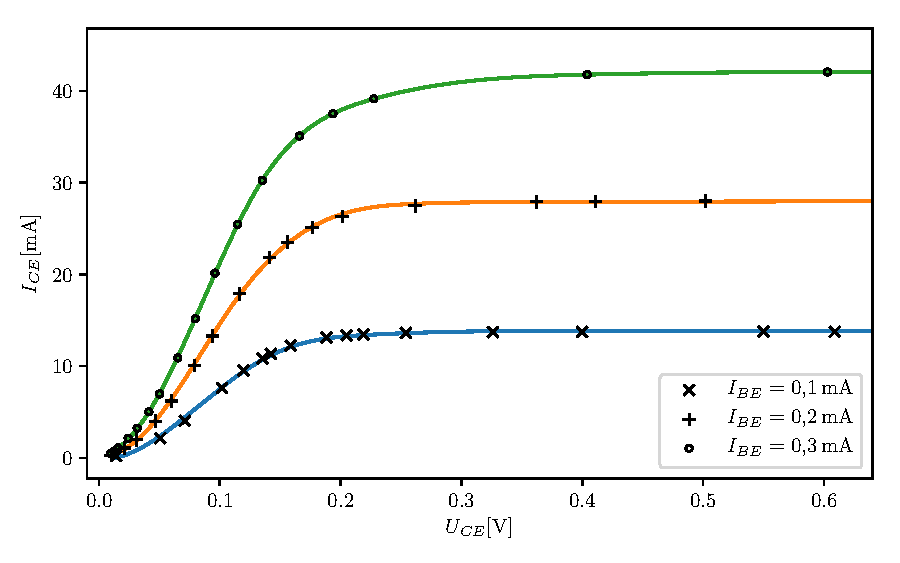
\includegraphics[]{u2}
\caption{Závislost Hallova napětí na magnetické indukci}
\label{fig:u2}
\end{figure}

\subsection*{Úkol 3}
Hodnoty chyb spočtených veličin v tomto a následujícím úkolu byly určeny metodou přenosu chyb.

Vodivost $\sigma$ byla určena podle \eqref{eq:sigma} jako 
$$\sigma = \SI{5,30 \pm 0,04}{\siemens\per\metre}.$$

Hallovu konstantu vzorku jsem spočítal podle \eqref{eq:R_H} pro oba konstantní proudy.
$$R_{H_{I = \SI{1}{A}}} = \SI{64,7 \pm 2,7 e-3}{\cubic\metre\per\ampere\per\second},$$
$$R_{H_{I = \SI{4,5}{A}}} = \SI{60,9 \pm 0,9 e-3}{\cubic\metre\per\ampere\per\second}.$$

Dále budeme počítat s průměrem těchto hodnot:
$$R_H = \SI{62,8 \pm 1,0 e-3}{\cubic\metre\per\ampere\per\second}$$.

\subsection*{Úkol 4}
Koncentraci nositelů náboje spočítáme z \eqref{eq:n}
$$n = \SI{1.171 \pm 0.012 e+20}{\per\cubic\metre}$$
a jejich pohyblivost podle \eqref{eq:mu_n}
$$\mu_n = \SI{0.2824 \pm 0.0022}{\cubic\metre\per\ohm\per\coulomb}.$$

\end{document}
